% Created by tikzDevice version 0.12 on 2019-03-12 12:51:37
% !TEX encoding = UTF-8 Unicode
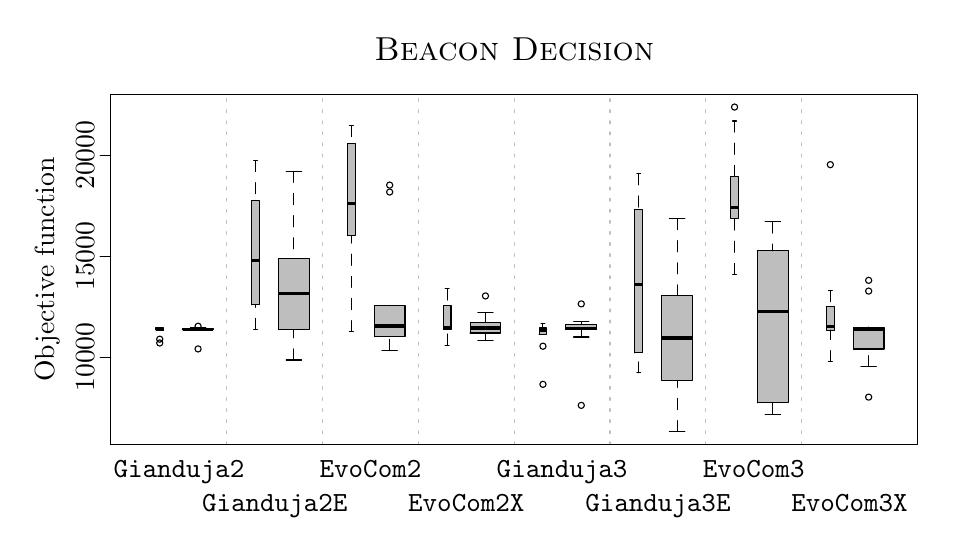
\begin{tikzpicture}[x=1pt,y=1pt]
\definecolor{fillColor}{RGB}{255,255,255}
\path[use as bounding box,fill=fillColor,fill opacity=0.00] (0,0) rectangle (325.21,180.67);
\begin{scope}
\path[clip] ( 30.00, 30.00) rectangle (321.61,156.67);
\definecolor{fillColor}{RGB}{190,190,190}

\path[fill=fillColor] ( 46.34, 71.46) --
	( 49.11, 71.46) --
	( 49.11, 72.13) --
	( 46.34, 72.13) --
	cycle;
\definecolor{drawColor}{RGB}{0,0,0}

\path[draw=drawColor,line width= 1.2pt,line join=round] ( 46.34, 71.58) -- ( 49.11, 71.58);

\path[draw=drawColor,line width= 0.4pt,dash pattern=on 4pt off 4pt ,line join=round,line cap=round] ( 47.72, 71.46) -- ( 47.72, 71.46);

\path[draw=drawColor,line width= 0.4pt,dash pattern=on 4pt off 4pt ,line join=round,line cap=round] ( 47.72, 72.16) -- ( 47.72, 72.13);

\path[draw=drawColor,line width= 0.4pt,line join=round,line cap=round] ( 47.03, 71.46) -- ( 48.42, 71.46);

\path[draw=drawColor,line width= 0.4pt,line join=round,line cap=round] ( 47.03, 72.16) -- ( 48.42, 72.16);

\path[draw=drawColor,line width= 0.4pt,line join=round,line cap=round] ( 46.34, 71.46) --
	( 49.11, 71.46) --
	( 49.11, 72.13) --
	( 46.34, 72.13) --
	( 46.34, 71.46);

\path[draw=drawColor,line width= 0.4pt,line join=round,line cap=round] ( 47.72, 66.73) circle (  1.12);

\path[draw=drawColor,line width= 0.4pt,line join=round,line cap=round] ( 47.72, 68.11) circle (  1.12);

\path[fill=fillColor] ( 56.03, 71.46) --
	( 67.11, 71.46) --
	( 67.11, 71.99) --
	( 56.03, 71.99) --
	cycle;

\path[draw=drawColor,line width= 1.2pt,line join=round] ( 56.03, 71.58) -- ( 67.11, 71.58);

\path[draw=drawColor,line width= 0.4pt,dash pattern=on 4pt off 4pt ,line join=round,line cap=round] ( 61.57, 71.35) -- ( 61.57, 71.46);

\path[draw=drawColor,line width= 0.4pt,dash pattern=on 4pt off 4pt ,line join=round,line cap=round] ( 61.57, 72.21) -- ( 61.57, 71.99);

\path[draw=drawColor,line width= 0.4pt,line join=round,line cap=round] ( 58.80, 71.35) -- ( 64.34, 71.35);

\path[draw=drawColor,line width= 0.4pt,line join=round,line cap=round] ( 58.80, 72.21) -- ( 64.34, 72.21);

\path[draw=drawColor,line width= 0.4pt,line join=round,line cap=round] ( 56.03, 71.46) --
	( 67.11, 71.46) --
	( 67.11, 71.99) --
	( 56.03, 71.99) --
	( 56.03, 71.46);

\path[draw=drawColor,line width= 0.4pt,line join=round,line cap=round] ( 61.57, 64.59) circle (  1.12);

\path[draw=drawColor,line width= 0.4pt,line join=round,line cap=round] ( 61.57, 72.78) circle (  1.12);

\path[fill=fillColor] ( 80.96, 80.48) --
	( 83.73, 80.48) --
	( 83.73,118.27) --
	( 80.96,118.27) --
	cycle;

\path[draw=drawColor,line width= 1.2pt,line join=round] ( 80.96, 96.51) -- ( 83.73, 96.51);

\path[draw=drawColor,line width= 0.4pt,dash pattern=on 4pt off 4pt ,line join=round,line cap=round] ( 82.34, 71.58) -- ( 82.34, 80.48);

\path[draw=drawColor,line width= 0.4pt,dash pattern=on 4pt off 4pt ,line join=round,line cap=round] ( 82.34,132.68) -- ( 82.34,118.27);

\path[draw=drawColor,line width= 0.4pt,line join=round,line cap=round] ( 81.65, 71.58) -- ( 83.03, 71.58);

\path[draw=drawColor,line width= 0.4pt,line join=round,line cap=round] ( 81.65,132.68) -- ( 83.03,132.68);

\path[draw=drawColor,line width= 0.4pt,line join=round,line cap=round] ( 80.96, 80.48) --
	( 83.73, 80.48) --
	( 83.73,118.27) --
	( 80.96,118.27) --
	( 80.96, 80.48);

\path[fill=fillColor] ( 90.65, 71.58) --
	(101.73, 71.58) --
	(101.73, 97.27) --
	( 90.65, 97.27) --
	cycle;

\path[draw=drawColor,line width= 1.2pt,line join=round] ( 90.65, 84.72) -- (101.73, 84.72);

\path[draw=drawColor,line width= 0.4pt,dash pattern=on 4pt off 4pt ,line join=round,line cap=round] ( 96.19, 60.58) -- ( 96.19, 71.58);

\path[draw=drawColor,line width= 0.4pt,dash pattern=on 4pt off 4pt ,line join=round,line cap=round] ( 96.19,128.74) -- ( 96.19, 97.27);

\path[draw=drawColor,line width= 0.4pt,line join=round,line cap=round] ( 93.42, 60.58) -- ( 98.96, 60.58);

\path[draw=drawColor,line width= 0.4pt,line join=round,line cap=round] ( 93.42,128.74) -- ( 98.96,128.74);

\path[draw=drawColor,line width= 0.4pt,line join=round,line cap=round] ( 90.65, 71.58) --
	(101.73, 71.58) --
	(101.73, 97.27) --
	( 90.65, 97.27) --
	( 90.65, 71.58);

\path[fill=fillColor] (115.57,105.50) --
	(118.34,105.50) --
	(118.34,138.71) --
	(115.57,138.71) --
	cycle;

\path[draw=drawColor,line width= 1.2pt,line join=round] (115.57,117.05) -- (118.34,117.05);

\path[draw=drawColor,line width= 0.4pt,dash pattern=on 4pt off 4pt ,line join=round,line cap=round] (116.96, 70.81) -- (116.96,105.50);

\path[draw=drawColor,line width= 0.4pt,dash pattern=on 4pt off 4pt ,line join=round,line cap=round] (116.96,145.31) -- (116.96,138.71);

\path[draw=drawColor,line width= 0.4pt,line join=round,line cap=round] (116.27, 70.81) -- (117.65, 70.81);

\path[draw=drawColor,line width= 0.4pt,line join=round,line cap=round] (116.27,145.31) -- (117.65,145.31);

\path[draw=drawColor,line width= 0.4pt,line join=round,line cap=round] (115.57,105.50) --
	(118.34,105.50) --
	(118.34,138.71) --
	(115.57,138.71) --
	(115.57,105.50);

\path[fill=fillColor] (125.27, 69.04) --
	(136.34, 69.04) --
	(136.34, 80.34) --
	(125.27, 80.34) --
	cycle;

\path[draw=drawColor,line width= 1.2pt,line join=round] (125.27, 72.87) -- (136.34, 72.87);

\path[draw=drawColor,line width= 0.4pt,dash pattern=on 4pt off 4pt ,line join=round,line cap=round] (130.81, 64.03) -- (130.81, 69.04);

\path[draw=drawColor,line width= 0.4pt,dash pattern=on 4pt off 4pt ,line join=round,line cap=round] (130.81, 80.34) -- (130.81, 80.34);

\path[draw=drawColor,line width= 0.4pt,line join=round,line cap=round] (128.04, 64.03) -- (133.57, 64.03);

\path[draw=drawColor,line width= 0.4pt,line join=round,line cap=round] (128.04, 80.34) -- (133.57, 80.34);

\path[draw=drawColor,line width= 0.4pt,line join=round,line cap=round] (125.27, 69.04) --
	(136.34, 69.04) --
	(136.34, 80.34) --
	(125.27, 80.34) --
	(125.27, 69.04);

\path[draw=drawColor,line width= 0.4pt,line join=round,line cap=round] (130.81,123.78) circle (  1.12);

\path[draw=drawColor,line width= 0.4pt,line join=round,line cap=round] (130.81,121.27) circle (  1.12);

\path[fill=fillColor] (150.19, 71.70) --
	(152.96, 71.70) --
	(152.96, 80.24) --
	(150.19, 80.24) --
	cycle;

\path[draw=drawColor,line width= 1.2pt,line join=round] (150.19, 72.26) -- (152.96, 72.26);

\path[draw=drawColor,line width= 0.4pt,dash pattern=on 4pt off 4pt ,line join=round,line cap=round] (151.58, 65.97) -- (151.58, 71.70);

\path[draw=drawColor,line width= 0.4pt,dash pattern=on 4pt off 4pt ,line join=round,line cap=round] (151.58, 86.26) -- (151.58, 80.24);

\path[draw=drawColor,line width= 0.4pt,line join=round,line cap=round] (150.88, 65.97) -- (152.27, 65.97);

\path[draw=drawColor,line width= 0.4pt,line join=round,line cap=round] (150.88, 86.26) -- (152.27, 86.26);

\path[draw=drawColor,line width= 0.4pt,line join=round,line cap=round] (150.19, 71.70) --
	(152.96, 71.70) --
	(152.96, 80.24) --
	(150.19, 80.24) --
	(150.19, 71.70);

\path[fill=fillColor] (159.88, 70.32) --
	(170.96, 70.32) --
	(170.96, 74.21) --
	(159.88, 74.21) --
	cycle;

\path[draw=drawColor,line width= 1.2pt,line join=round] (159.88, 72.16) -- (170.96, 72.16);

\path[draw=drawColor,line width= 0.4pt,dash pattern=on 4pt off 4pt ,line join=round,line cap=round] (165.42, 67.58) -- (165.42, 70.32);

\path[draw=drawColor,line width= 0.4pt,dash pattern=on 4pt off 4pt ,line join=round,line cap=round] (165.42, 77.70) -- (165.42, 74.21);

\path[draw=drawColor,line width= 0.4pt,line join=round,line cap=round] (162.65, 67.58) -- (168.19, 67.58);

\path[draw=drawColor,line width= 0.4pt,line join=round,line cap=round] (162.65, 77.70) -- (168.19, 77.70);

\path[draw=drawColor,line width= 0.4pt,line join=round,line cap=round] (159.88, 70.32) --
	(170.96, 70.32) --
	(170.96, 74.21) --
	(159.88, 74.21) --
	(159.88, 70.32);

\path[draw=drawColor,line width= 0.4pt,line join=round,line cap=round] (165.42, 83.74) circle (  1.12);

\path[fill=fillColor] (184.81, 69.86) --
	(187.58, 69.86) --
	(187.58, 72.13) --
	(184.81, 72.13) --
	cycle;

\path[draw=drawColor,line width= 1.2pt,line join=round] (184.81, 71.34) -- (187.58, 71.34);

\path[draw=drawColor,line width= 0.4pt,dash pattern=on 4pt off 4pt ,line join=round,line cap=round] (186.19, 69.86) -- (186.19, 69.86);

\path[draw=drawColor,line width= 0.4pt,dash pattern=on 4pt off 4pt ,line join=round,line cap=round] (186.19, 73.62) -- (186.19, 72.13);

\path[draw=drawColor,line width= 0.4pt,line join=round,line cap=round] (185.50, 69.86) -- (186.88, 69.86);

\path[draw=drawColor,line width= 0.4pt,line join=round,line cap=round] (185.50, 73.62) -- (186.88, 73.62);

\path[draw=drawColor,line width= 0.4pt,line join=round,line cap=round] (184.81, 69.86) --
	(187.58, 69.86) --
	(187.58, 72.13) --
	(184.81, 72.13) --
	(184.81, 69.86);

\path[draw=drawColor,line width= 0.4pt,line join=round,line cap=round] (186.19, 51.79) circle (  1.12);

\path[draw=drawColor,line width= 0.4pt,line join=round,line cap=round] (186.19, 65.57) circle (  1.12);

\path[fill=fillColor] (194.50, 71.58) --
	(205.58, 71.58) --
	(205.58, 73.56) --
	(194.50, 73.56) --
	cycle;

\path[draw=drawColor,line width= 1.2pt,line join=round] (194.50, 71.95) -- (205.58, 71.95);

\path[draw=drawColor,line width= 0.4pt,dash pattern=on 4pt off 4pt ,line join=round,line cap=round] (200.04, 68.89) -- (200.04, 71.58);

\path[draw=drawColor,line width= 0.4pt,dash pattern=on 4pt off 4pt ,line join=round,line cap=round] (200.04, 74.43) -- (200.04, 73.56);

\path[draw=drawColor,line width= 0.4pt,line join=round,line cap=round] (197.27, 68.89) -- (202.81, 68.89);

\path[draw=drawColor,line width= 0.4pt,line join=round,line cap=round] (197.27, 74.43) -- (202.81, 74.43);

\path[draw=drawColor,line width= 0.4pt,line join=round,line cap=round] (194.50, 71.58) --
	(205.58, 71.58) --
	(205.58, 73.56) --
	(194.50, 73.56) --
	(194.50, 71.58);

\path[draw=drawColor,line width= 0.4pt,line join=round,line cap=round] (200.04, 44.19) circle (  1.12);

\path[draw=drawColor,line width= 0.4pt,line join=round,line cap=round] (200.04, 80.86) circle (  1.12);

\path[fill=fillColor] (219.43, 63.19) --
	(222.19, 63.19) --
	(222.19,114.93) --
	(219.43,114.93) --
	cycle;

\path[draw=drawColor,line width= 1.2pt,line join=round] (219.43, 87.89) -- (222.19, 87.89);

\path[draw=drawColor,line width= 0.4pt,dash pattern=on 4pt off 4pt ,line join=round,line cap=round] (220.81, 55.91) -- (220.81, 63.19);

\path[draw=drawColor,line width= 0.4pt,dash pattern=on 4pt off 4pt ,line join=round,line cap=round] (220.81,127.84) -- (220.81,114.93);

\path[draw=drawColor,line width= 0.4pt,line join=round,line cap=round] (220.12, 55.91) -- (221.50, 55.91);

\path[draw=drawColor,line width= 0.4pt,line join=round,line cap=round] (220.12,127.84) -- (221.50,127.84);

\path[draw=drawColor,line width= 0.4pt,line join=round,line cap=round] (219.43, 63.19) --
	(222.19, 63.19) --
	(222.19,114.93) --
	(219.43,114.93) --
	(219.43, 63.19);

\path[fill=fillColor] (229.12, 53.21) --
	(240.20, 53.21) --
	(240.20, 84.00) --
	(229.12, 84.00) --
	cycle;

\path[draw=drawColor,line width= 1.2pt,line join=round] (229.12, 68.59) -- (240.20, 68.59);

\path[draw=drawColor,line width= 0.4pt,dash pattern=on 4pt off 4pt ,line join=round,line cap=round] (234.66, 34.69) -- (234.66, 53.21);

\path[draw=drawColor,line width= 0.4pt,dash pattern=on 4pt off 4pt ,line join=round,line cap=round] (234.66,111.70) -- (234.66, 84.00);

\path[draw=drawColor,line width= 0.4pt,line join=round,line cap=round] (231.89, 34.69) -- (237.43, 34.69);

\path[draw=drawColor,line width= 0.4pt,line join=round,line cap=round] (231.89,111.70) -- (237.43,111.70);

\path[draw=drawColor,line width= 0.4pt,line join=round,line cap=round] (229.12, 53.21) --
	(240.20, 53.21) --
	(240.20, 84.00) --
	(229.12, 84.00) --
	(229.12, 53.21);

\path[fill=fillColor] (254.04,111.80) --
	(256.81,111.80) --
	(256.81,127.04) --
	(254.04,127.04) --
	cycle;

\path[draw=drawColor,line width= 1.2pt,line join=round] (254.04,115.65) -- (256.81,115.65);

\path[draw=drawColor,line width= 0.4pt,dash pattern=on 4pt off 4pt ,line join=round,line cap=round] (255.43, 91.52) -- (255.43,111.80);

\path[draw=drawColor,line width= 0.4pt,dash pattern=on 4pt off 4pt ,line join=round,line cap=round] (255.43,146.93) -- (255.43,127.04);

\path[draw=drawColor,line width= 0.4pt,line join=round,line cap=round] (254.73, 91.52) -- (256.12, 91.52);

\path[draw=drawColor,line width= 0.4pt,line join=round,line cap=round] (254.73,146.93) -- (256.12,146.93);

\path[draw=drawColor,line width= 0.4pt,line join=round,line cap=round] (254.04,111.80) --
	(256.81,111.80) --
	(256.81,127.04) --
	(254.04,127.04) --
	(254.04,111.80);

\path[draw=drawColor,line width= 0.4pt,line join=round,line cap=round] (255.43,151.98) circle (  1.12);

\path[fill=fillColor] (263.74, 45.12) --
	(274.81, 45.12) --
	(274.81,100.06) --
	(263.74,100.06) --
	cycle;

\path[draw=drawColor,line width= 1.2pt,line join=round] (263.74, 78.06) -- (274.81, 78.06);

\path[draw=drawColor,line width= 0.4pt,dash pattern=on 4pt off 4pt ,line join=round,line cap=round] (269.27, 40.92) -- (269.27, 45.12);

\path[draw=drawColor,line width= 0.4pt,dash pattern=on 4pt off 4pt ,line join=round,line cap=round] (269.27,110.48) -- (269.27,100.06);

\path[draw=drawColor,line width= 0.4pt,line join=round,line cap=round] (266.50, 40.92) -- (272.04, 40.92);

\path[draw=drawColor,line width= 0.4pt,line join=round,line cap=round] (266.50,110.48) -- (272.04,110.48);

\path[draw=drawColor,line width= 0.4pt,line join=round,line cap=round] (263.74, 45.12) --
	(274.81, 45.12) --
	(274.81,100.06) --
	(263.74,100.06) --
	(263.74, 45.12);

\path[fill=fillColor] (288.66, 71.38) --
	(291.43, 71.38) --
	(291.43, 80.00) --
	(288.66, 80.00) --
	cycle;

\path[draw=drawColor,line width= 1.2pt,line join=round] (288.66, 72.57) -- (291.43, 72.57);

\path[draw=drawColor,line width= 0.4pt,dash pattern=on 4pt off 4pt ,line join=round,line cap=round] (290.04, 59.97) -- (290.04, 71.38);

\path[draw=drawColor,line width= 0.4pt,dash pattern=on 4pt off 4pt ,line join=round,line cap=round] (290.04, 85.71) -- (290.04, 80.00);

\path[draw=drawColor,line width= 0.4pt,line join=round,line cap=round] (289.35, 59.97) -- (290.74, 59.97);

\path[draw=drawColor,line width= 0.4pt,line join=round,line cap=round] (289.35, 85.71) -- (290.74, 85.71);

\path[draw=drawColor,line width= 0.4pt,line join=round,line cap=round] (288.66, 71.38) --
	(291.43, 71.38) --
	(291.43, 80.00) --
	(288.66, 80.00) --
	(288.66, 71.38);

\path[draw=drawColor,line width= 0.4pt,line join=round,line cap=round] (290.04,131.17) circle (  1.12);

\path[fill=fillColor] (298.35, 64.57) --
	(309.43, 64.57) --
	(309.43, 72.47) --
	(298.35, 72.47) --
	cycle;

\path[draw=drawColor,line width= 1.2pt,line join=round] (298.35, 71.61) -- (309.43, 71.61);

\path[draw=drawColor,line width= 0.4pt,dash pattern=on 4pt off 4pt ,line join=round,line cap=round] (303.89, 58.19) -- (303.89, 64.57);

\path[draw=drawColor,line width= 0.4pt,dash pattern=on 4pt off 4pt ,line join=round,line cap=round] (303.89, 72.47) -- (303.89, 72.47);

\path[draw=drawColor,line width= 0.4pt,line join=round,line cap=round] (301.12, 58.19) -- (306.66, 58.19);

\path[draw=drawColor,line width= 0.4pt,line join=round,line cap=round] (301.12, 72.47) -- (306.66, 72.47);

\path[draw=drawColor,line width= 0.4pt,line join=round,line cap=round] (298.35, 64.57) --
	(309.43, 64.57) --
	(309.43, 72.47) --
	(298.35, 72.47) --
	(298.35, 64.57);

\path[draw=drawColor,line width= 0.4pt,line join=round,line cap=round] (303.89, 89.36) circle (  1.12);

\path[draw=drawColor,line width= 0.4pt,line join=round,line cap=round] (303.89, 47.17) circle (  1.12);

\path[draw=drawColor,line width= 0.4pt,line join=round,line cap=round] (303.89, 85.48) circle (  1.12);
\definecolor{drawColor}{RGB}{190,190,190}

\path[draw=drawColor,line width= 0.4pt,dash pattern=on 1pt off 3pt ,line join=round,line cap=round] ( 71.96, 30.00) -- ( 71.96,156.67);

\path[draw=drawColor,line width= 0.4pt,dash pattern=on 1pt off 3pt ,line join=round,line cap=round] (106.57, 30.00) -- (106.57,156.67);

\path[draw=drawColor,line width= 0.4pt,dash pattern=on 1pt off 3pt ,line join=round,line cap=round] (141.19, 30.00) -- (141.19,156.67);

\path[draw=drawColor,line width= 0.4pt,dash pattern=on 1pt off 3pt ,line join=round,line cap=round] (175.81, 30.00) -- (175.81,156.67);

\path[draw=drawColor,line width= 0.4pt,dash pattern=on 1pt off 3pt ,line join=round,line cap=round] (210.42, 30.00) -- (210.42,156.67);

\path[draw=drawColor,line width= 0.4pt,dash pattern=on 1pt off 3pt ,line join=round,line cap=round] (245.04, 30.00) -- (245.04,156.67);

\path[draw=drawColor,line width= 0.4pt,dash pattern=on 1pt off 3pt ,line join=round,line cap=round] (279.66, 30.00) -- (279.66,156.67);
\end{scope}
\begin{scope}
\path[clip] (  0.00,  0.00) rectangle (325.21,180.67);
\definecolor{drawColor}{RGB}{0,0,0}

\node[text=drawColor,anchor=base,inner sep=0pt, outer sep=0pt, scale=  1.00] at ( 54.65, 18.00) {\texttt{Gianduja2}};

\node[text=drawColor,anchor=base,inner sep=0pt, outer sep=0pt, scale=  1.00] at (123.88, 18.00) {\texttt{EvoCom2}};

\node[text=drawColor,anchor=base,inner sep=0pt, outer sep=0pt, scale=  1.00] at (193.12, 18.00) {\texttt{Gianduja3}};

\node[text=drawColor,anchor=base,inner sep=0pt, outer sep=0pt, scale=  1.00] at (262.35, 18.00) {\texttt{EvoCom3}};

\node[text=drawColor,anchor=base,inner sep=0pt, outer sep=0pt, scale=  1.00] at ( 89.26,  6.00) {\texttt{Gianduja2E}};

\node[text=drawColor,anchor=base,inner sep=0pt, outer sep=0pt, scale=  1.00] at (158.50,  6.00) {\texttt{EvoCom2X}};

\node[text=drawColor,anchor=base,inner sep=0pt, outer sep=0pt, scale=  1.00] at (227.73,  6.00) {\texttt{Gianduja3E}};

\node[text=drawColor,anchor=base,inner sep=0pt, outer sep=0pt, scale=  1.00] at (296.97,  6.00) {\texttt{EvoCom3X}};
\end{scope}
\begin{scope}
\path[clip] (  0.00,  0.00) rectangle (325.21,180.67);
\definecolor{drawColor}{RGB}{0,0,0}

\node[text=drawColor,anchor=base,inner sep=0pt, outer sep=0pt, scale=  1.20] at (175.81,168.67) {\textsc{Beacon Decision}};

\node[text=drawColor,rotate= 90.00,anchor=base,inner sep=0pt, outer sep=0pt, scale=  1.00] at (  9.60, 93.34) {Objective function};
\end{scope}
\begin{scope}
\path[clip] (  0.00,  0.00) rectangle (325.21,180.67);
\definecolor{drawColor}{RGB}{0,0,0}

\path[draw=drawColor,line width= 0.4pt,line join=round,line cap=round] ( 30.00, 61.64) -- ( 30.00,134.63);

\path[draw=drawColor,line width= 0.4pt,line join=round,line cap=round] ( 30.00, 61.64) -- ( 26.20, 61.64);

\path[draw=drawColor,line width= 0.4pt,line join=round,line cap=round] ( 30.00, 98.13) -- ( 26.20, 98.13);

\path[draw=drawColor,line width= 0.4pt,line join=round,line cap=round] ( 30.00,134.63) -- ( 26.20,134.63);

\node[text=drawColor,rotate= 90.00,anchor=base,inner sep=0pt, outer sep=0pt, scale=  1.00] at ( 24.00, 61.64) {10000};

\node[text=drawColor,rotate= 90.00,anchor=base,inner sep=0pt, outer sep=0pt, scale=  1.00] at ( 24.00, 98.13) {15000};

\node[text=drawColor,rotate= 90.00,anchor=base,inner sep=0pt, outer sep=0pt, scale=  1.00] at ( 24.00,134.63) {20000};

\path[draw=drawColor,line width= 0.4pt,line join=round,line cap=round] ( 30.00, 30.00) --
	(321.61, 30.00) --
	(321.61,156.67) --
	( 30.00,156.67) --
	( 30.00, 30.00);
\end{scope}
\end{tikzpicture}
